\chapter{Stopwatch Datapath}
\label{chapter:stopDatapath}
\graphicspath{ {./Lab09Datapath/Fig} }



\section{Outcomes and Objectives}

The outcome of this lab is to design and simulate 
a datapath to store and manipulate the information need to run a stopwatch.
Through this process you will achieve the following
learning objectives.
\begin{itemize}
	\item \Paste{bok:BMS_RegTran}
	\item \Paste{bok:DaC_Architecture}
	\item \Paste{bok:DaC_ControWord}
	\item \Paste{HDL:Do}
\end{itemize}



\section{Stopwatch}

A stopwatch is a device that is used to measure time intervals, usually
in competitive events. The stopwatch that you will be designing gets its
input from two buttons. The stopwatch will measure down to a 1/10th of a
second. The time will be displayed using 3 digits which will represent
tenths of a second, unit second and tens of seconds. As a result, the
stopwatch is limited to measuring intervals of time from 0.1 second to
99.9 seconds.

The stopwatch's behavior is dictated by its 2 buttons called S1 and S2
according to the finite state machine shown in Figure~\ref{fig:swDPbehavior}.

\begin{figure}[ht]
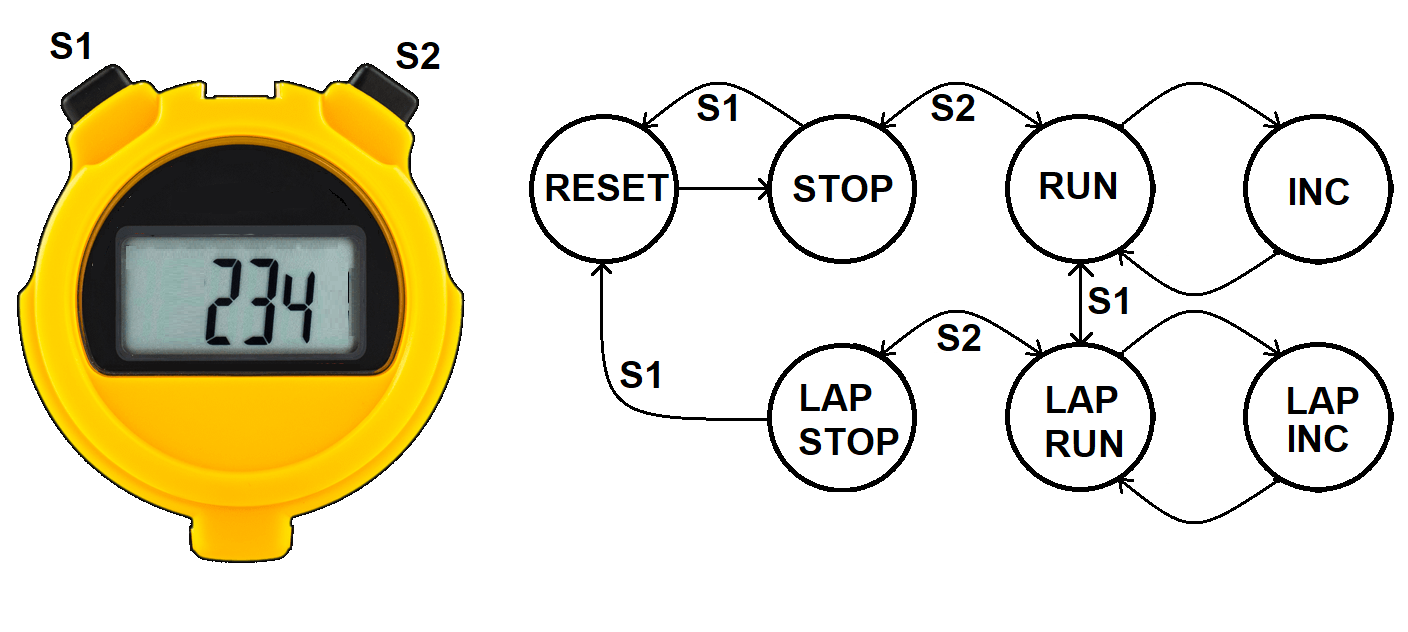
\includegraphics[width=0.5\paperwidth]{image1.png}
\caption{A digital stopwatch gets its input from 2 buttons and displays
its output on a 7-segment display. The behavior of the stopwatch can be
described by this finite state machine (FSM).}
\label{fig:swDPbehavior}
\end{figure}

To make sense out of the FSM shown in Figure~\ref{fig:swDPbehavior}, its helpful to imagine
timing a 4-person relay race. In this race, each athlete runs one lap
and then pass a baton to the next runner. The time required for a runner
to complete one lap is called their split time. In order to measure each
runner's split time, you need to be able to stop the displayed time
while allowing the stopwatch to continue to run its internal timer. This
is called a lap feature. Let's explore how the lap feature works by
timing the mile relay at a Mines track meet. As we go through this
scenario, reference the finite state machine in Figure~\ref{fig:swDPbehavior}.

Prior to the start of the race, you push button S1 putting the stopwatch
into the RESET state. This clears the internal timer and the displayed
time. The stopwatch automatically goes back to the STOP state. You are
ready for the start of the race. You are ready when the gun goes off and
immediately press button S2 putting the stopwatch into the RUN state.
The internal timer is keeping track of the elapsed time and you this the
displayed time changing to reflect the internal timer. As soon as the
first runner who is finishing their lap hands the baton to the second
runner, you press button S1 putting the stopwatch into the LAP RUN
state. This causes the displayed time to stop, showing the time at the
instant you pressed button S1, while simultaneously allowing the
internal timer to keep running. The internal timer is now keeping track
of the elapsed time since the start of the race. You calmy write down
the displayed time on your clip board (made easier because it is not
changing) and then press button S1 putting the stopwatch back into the
RUN state. You repeat this process until the last runner comes in. As
soon as they do, you press button S2 stopping the internal timer and
showing the time the last runner crossed the finish line.

In this scenario we did not put the stopwatch into the LAP STOP state --
this state would stop the internal timer and keep the displayed time the
moment the S1 button was pressed when the stopwatch was in the RUN
state. You should also note, we did not talk about the INC and LAP INC
states. Let's explore them now.

Clearly, the stopwatch does not increment the stored and displayed time
at 50Mhz. The stored and displayed time count up every
10\textsuperscript{th} of a second. This is managed by the
counter/comparator at the top of Figure~\ref{fig:dpSWdatpath} which asserts the
\textbf{tenth} signal every 10\textsuperscript{th} of a second. This
signal tells the FSM in Figure~\ref{fig:swDPbehavior} to transition from the RUN state to the
INC state. In the INC state the stored time is incremented and the
counter at the top of Figure~\ref{fig:dpSWdatpath} is reset back to 0. The LAP INC state
performs a similar function for the LAP state.

To summarize:

\begin{itemize}
\item
  RESET -- Reset the internal and displayed time values.
\item
  STOP -- Stop the 10\textsuperscript{th} second timer and hold the
  displayed time.
\item
  RUN -- Run the 10\textsuperscript{th} second timer and display the
  stored time.
\item
  INC -- Increment the stored time
\item
  LAP RUN -- Run the 10\textsuperscript{th} second timer and hold the
  displayed time.
\item
  LAP INC - Increment the stored time.
\item
  LAP STOP -- Stop the 10\textsuperscript{th} second timer and hold the
  displayed time.
\end{itemize}

\section{Module: stopWatchDatapath}

The datapath for the stopwatch is shown in Figure~\ref{fig:dpSWdatpath}. The behavior of the
datapath to perform the functions of a stopwatch follows.

\begin{figure}[ht]
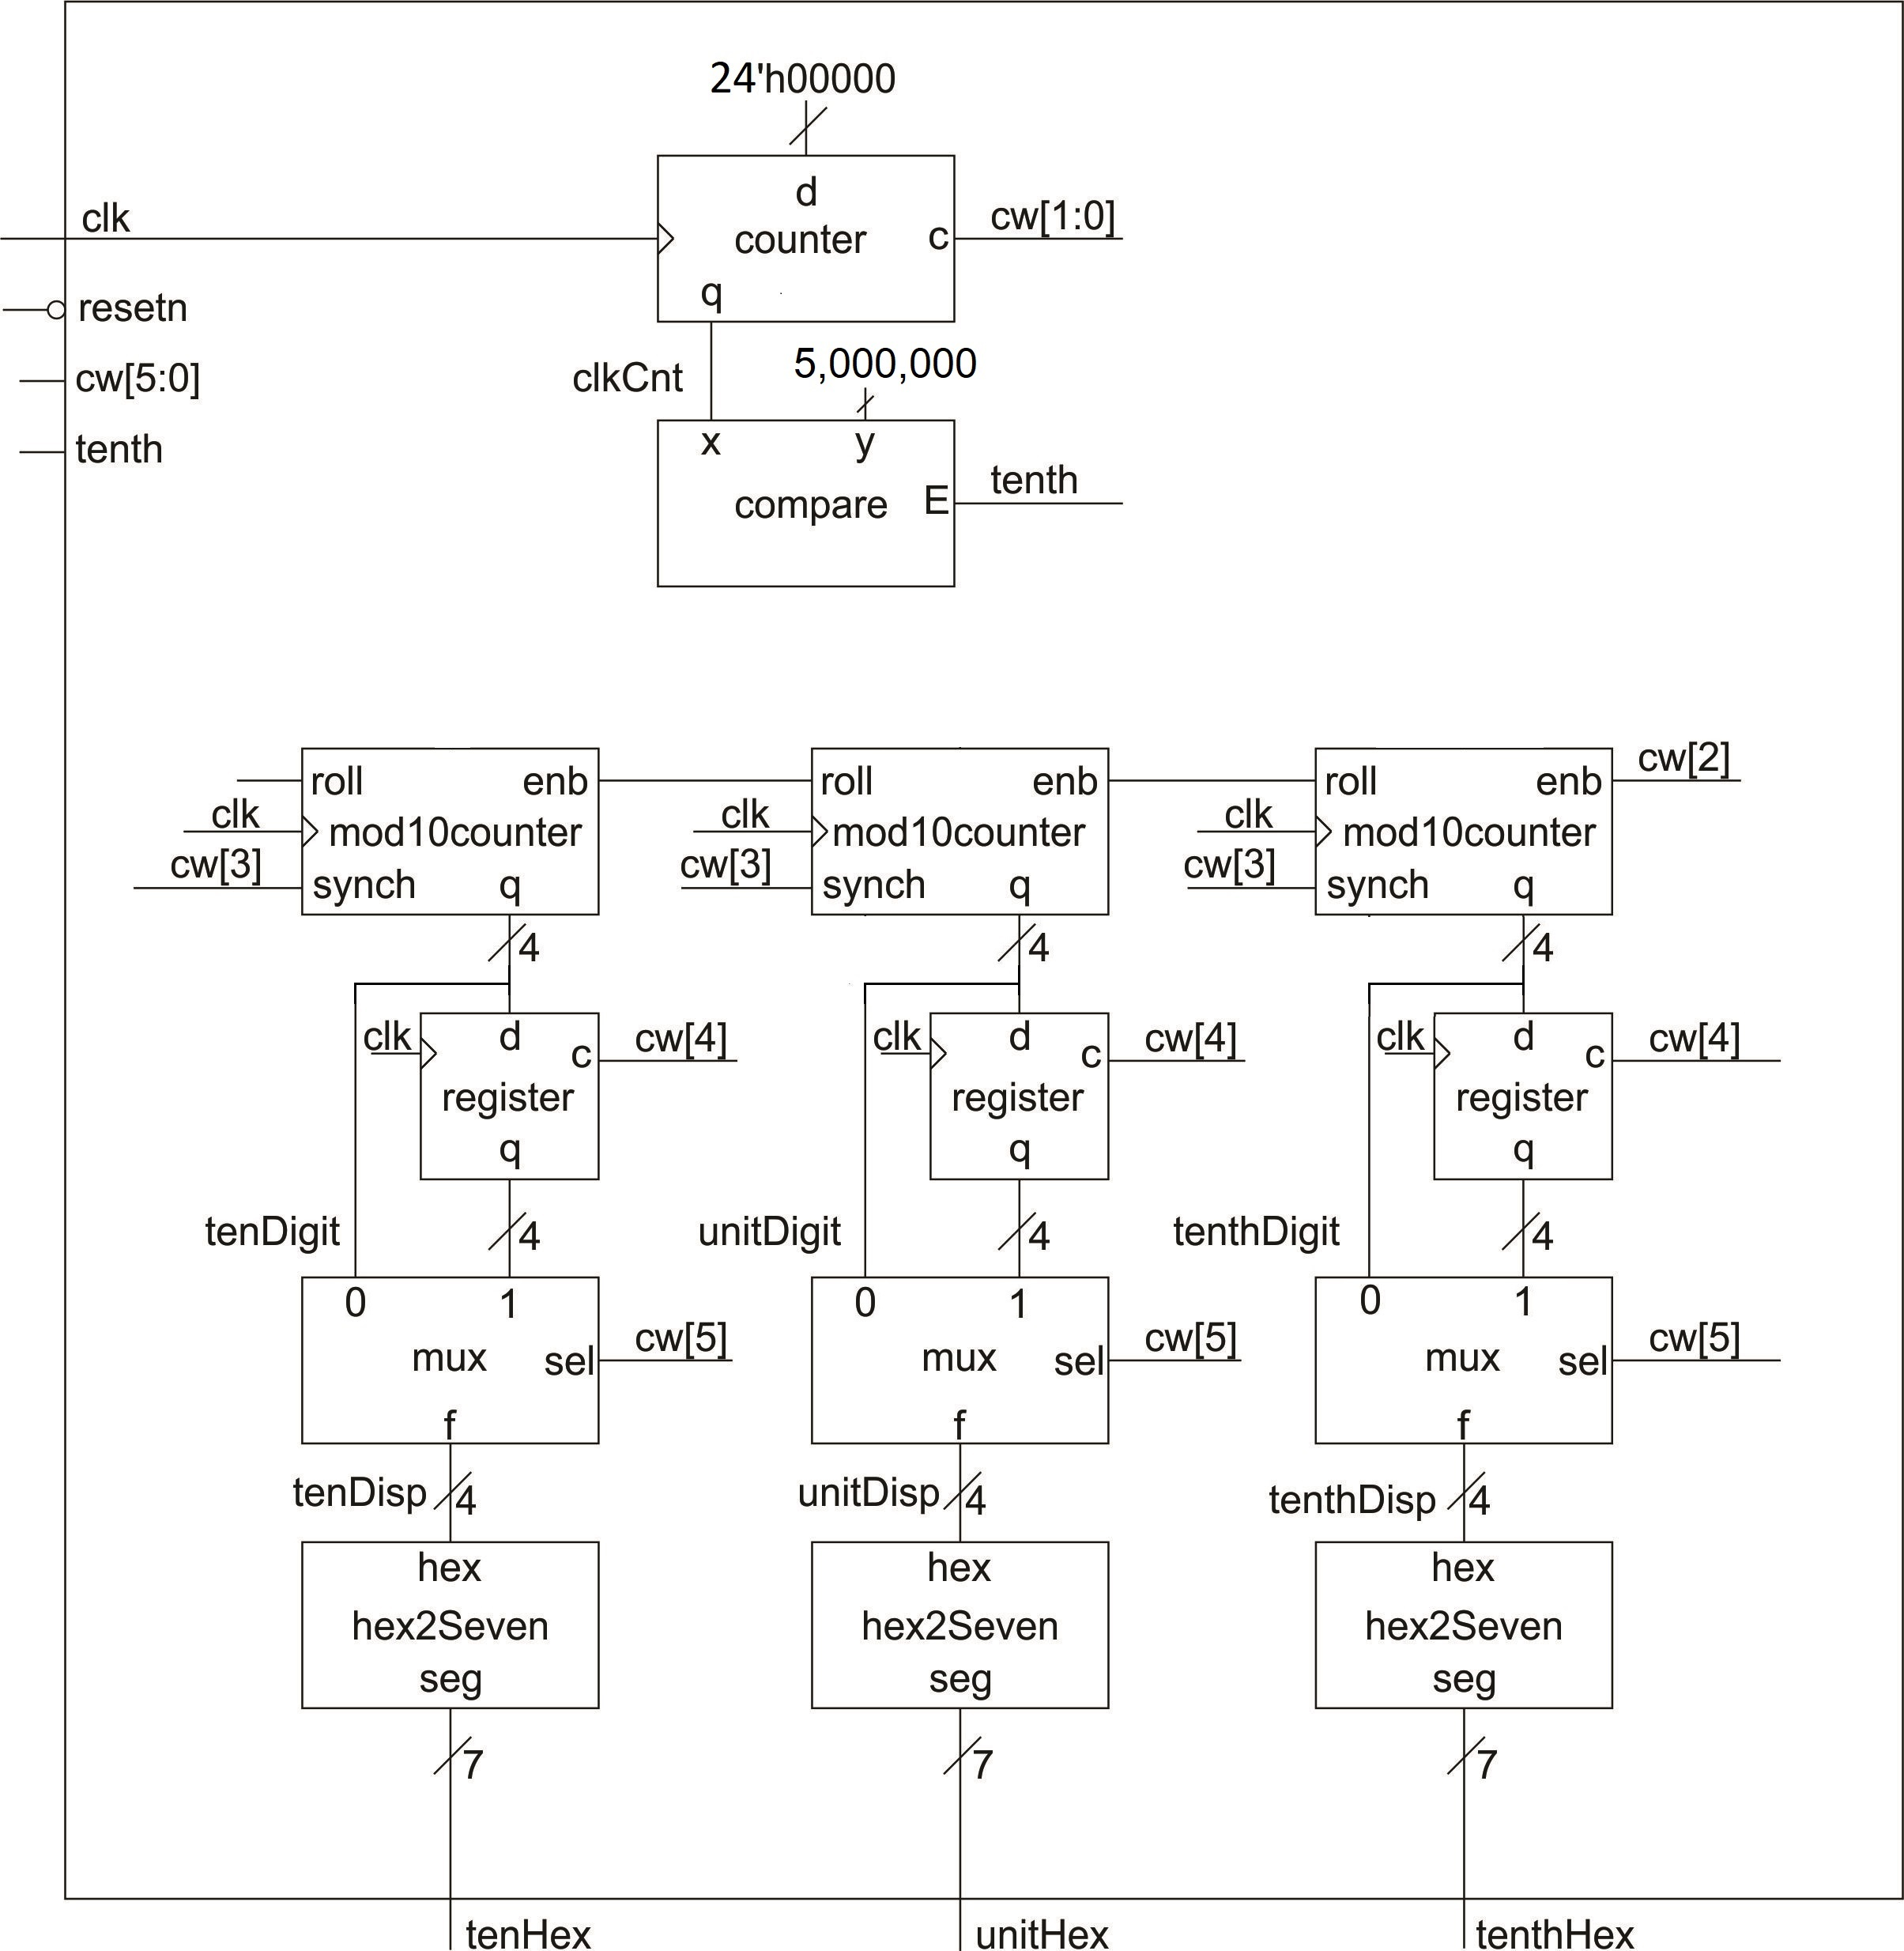
\includegraphics{ image2.jpg}
\caption{The datapath for the stopwatch has a 6-bit control word and
displays the time on three 7-segment displays.}
\label{fig:dpSWdatpath}
\end{figure}

The internal time is formed by the counter/comparator combination at the
top of Figure~\ref{fig:dpSWdatpath}. The \textbf{clk} input from the Development Board runs
at 50MHz. This will be the rate at which the \textbf{clkCnt} output from
counter counts up. When \textbf{clkCnt} counts from 0 to 5,000,000 then
1/10\textsuperscript{th} of a second has gone by. The \textbf{roll}
signal indicates when 1/10\textsuperscript{th} of a second has gone by.
The control unit you build will build in the next lab, will use this
signal to coordinate incrementing the bank of mod 10 counters in the
datapath. Note that the bank of mod 10 counters are incremented in a
state called INC, that is not shown in Figure~\ref{fig:swDPbehavior}. The output of the mod10
counters, \textbf{tenDigit}, \textbf{unitDigit} and \textbf{tenthDigit}
can be latched-up in the register bank so that the datapath can hold the
displayed time while still allowing the bank of mod 10 counters to keep
track of the elapsed time. The multiplexer controls what is displayed.
The 4-bit digit representing a time digit, \textbf{tenDisp},
\textbf{unitDisp} and \textbf{tenthDisp} are converted into a 7-segment
pattern before leaving the datapath.

To better understand the datapath, construct the control word for each
state. In order to help you, the actions associated with each state are
outlined below. In some cases, you will need to make decisions about the
control bits. Use your understanding of the datapath's operation and
your intuition of how you would want to the datapath to work. If this is
uncomfortable, please understand that it's important for you to learn
how to make design decisions on your own so that you can reach your full
potential as an engineer.

\begin{itemize}
\item
  RESET -- clear the values in the registers and counters
\item
  STOP -- hold the timer counter and display the mod 10 counters
\item
  RUN -- allow the timer counter to count up and display the mod 10
  counters
\item
  INC -- clear the timer counter and increment the mod 10 counters
\item
  RUN2LAP -- Latch up the mod 10 counters in the lap register
\item
  LAP RUN -- allow the timer counter to count up, display the latched
  time
\item
  LAP INC -- clear the timer counter and increment the mod 10 counters
\item
  LAP STOP -- stop the timer counter and display the latched time
\end{itemize}

\begin{longtable}[]{@{}
| >{\raggedright\arraybackslash}p{(\columnwidth - 10\tabcolsep) * \real{0.1666}}|
  >{\raggedright\arraybackslash}p{(\columnwidth - 10\tabcolsep) * \real{0.1666}}|
  >{\raggedright\arraybackslash}p{(\columnwidth - 10\tabcolsep) * \real{0.1666}}|
  >{\raggedright\arraybackslash}p{(\columnwidth - 10\tabcolsep) * \real{0.1666}}|
  >{\raggedright\arraybackslash}p{(\columnwidth - 10\tabcolsep) * \real{0.1667}}|
  >{\raggedright\arraybackslash}p{(\columnwidth - 10\tabcolsep) * \real{0.1667}}|@{}}
\caption{Control word table for the datapath shown in Figure~\ref{fig:dpSWdatpath}}
\label{table:swDPcontrolWord}\tabularnewline
\toprule()
\begin{minipage}[b]{\linewidth}\raggedright
\end{minipage} & \begin{minipage}[b]{\linewidth}\raggedright
\textbf{cw{[}5{]}}

\textbf{2x1 mux}
\end{minipage} & \begin{minipage}[b]{\linewidth}\raggedright
\textbf{cw{[}4{]}}

\textbf{lap register}
\end{minipage} & \begin{minipage}[b]{\linewidth}\raggedright
\textbf{cw{[}3{]}}

\textbf{mod10 reset}
\end{minipage} & \begin{minipage}[b]{\linewidth}\raggedright
\textbf{cw{[}2{]}}

\textbf{mod10 count}
\end{minipage} & \begin{minipage}[b]{\linewidth}\raggedright
\textbf{cw{[}1:0{]}}

\textbf{timer counter}
\end{minipage} \\
\midrule()
\endfirsthead
\toprule()
\begin{minipage}[b]{\linewidth}\raggedright
\end{minipage} & \begin{minipage}[b]{\linewidth}\raggedright
\textbf{cw{[}5{]}}

\textbf{2x1 mux}
\end{minipage} & \begin{minipage}[b]{\linewidth}\raggedright
\textbf{cw{[}4{]}}

\textbf{lap register}
\end{minipage} & \begin{minipage}[b]{\linewidth}\raggedright
\textbf{cw{[}3{]}}

\textbf{mod10 reset}
\end{minipage} & \begin{minipage}[b]{\linewidth}\raggedright
\textbf{cw{[}2{]}}

\textbf{mod10 count}
\end{minipage} & \begin{minipage}[b]{\linewidth}\raggedright
\textbf{cw{[}1:0{]}}

\textbf{timer counter}
\end{minipage} \\
\midrule()
\endhead
& 0 = mod10 & 1 = load & 1 = reset & 1 = count up & 11 = load \\ \hline
& 1 = register & 0 = hold & 0 = hold & 0 = hold & 10 = count up \\ \hline
& & & & & 01 = not used \\ \hline
& & & & & 00 = hold \\ \hline
\textbf{RESET} & & & 1 & & \\ \hline
\textbf{STOP} & & & & & \\ \hline
\textbf{RUN} & & & & & \\ \hline
\textbf{INC} & & & & & \\ \hline
\textbf{RUN2LAP} & & & & 0 & \\ \hline
\textbf{LAP RUN} & & & & & 10 \\ \hline
\textbf{LAP INC} & & 0 & & & \\ \hline
\textbf{LAP STOP} & 1 & & & & \\
\bottomrule()
\end{longtable}

\hypertarget{link:swDpVerilog}{}{}
Now that you have the control word figured out, you need to write the
Verilog code for the datapath. For the datapath module:

\begin{itemize}
\item
  Use the datapath.v file provided in the Canvas folder as the starting
  point.

  \begin{itemize}
  \item
    Use the module definitions from previous land and the Canvas lab
    folder for this lab.
  \end{itemize}
\item
  Provide meaningful names to the wires in the module.
\item
  Properly tab-indent your code

  \begin{itemize}
  \item
    Single level for wire declarations
  \item
    Single level for component instantiations
  \item
    Two levels for case statement
  \item
    Three levels for case values
  \end{itemize}
\end{itemize}

\section{Testbench}

Before you download your completed datapath to the Development Board,
you are going to perform extensive simulations to uncover as many bugs
as possible. Trust me, errors are much, much easier to find in a
simulation.

There is a practical consideration that will make the simulation more
manageable. The counter-comparator combination in Figure~\ref{fig:dpSWdatpath} acts as a
clock divider circuit. The counter counts up at 50MHz (the main
oscillator frequency). The comparator checks when the count reaches
5,000,000 = 0x4C4B40, meaning that a 1/10\textsuperscript{th} of a
second has gone by. You do not want to have to run the counter to
5,000,000 in your simulation, it would just take too long. To replace
the 5,000,000 constant you need to go into the datapath.v module and
modify the following:

\begin{itemize}
\item
Set \verb+ localparam tenthSecondConstant+ to 4\textquotesingle h000002
  (an arbitrary small constant)
\item
  Set the parameter \verb+N+ to 4, this sets the word size of the counter/comparator hardware.
\end{itemize}

You can use the parameter \textbf{N} as the generic parameter in
component instantiation for generic components. For example, 
you will have the following genericCounter instantiation in your 
datapath - the use of the parameter value \hdl{\#(N)} as the width of the 
counter is legal syntax in Verilog as long as \hdl{N} is defined somewhere.

\begin{verbatim}
genericCounter #(N) tenthSecondCounter(clk, resetn, zero24, cw{[}1:0{]}, clkCount);
\end{verbatim}

Make a note to yourself to modify \hdl{N} and
\hdl{tenthSecondConstant} values before synthesis. This is also
mentioned later in this document.

Next modify the control words defined in the datapathLab09\_tb.v file
using the values from Table~\ref{table:swDPcontrolWord}.

Finally, you need to understand what output the simulation should output
so that you can compare that to what your simulation actually producing.
Any difference between these two indicate an error (either in your
understanding or circuit behavior) that need to be fixed.

To do this complete the entries in the following timing diagram figures.
Use the code in the testbench to figure out the values for the control
word and how long they are held. The control word does not necessarily
change every 20ns. When it does not, you can just rewrite the control
word or edit the image to connect adjacent cells.

The \$display statement in the testbench prints out a message when that
line of the simulation is reached. Including these statements helps you
to understand where your simulation is at and what behavior to expect.

\begin{landscape}
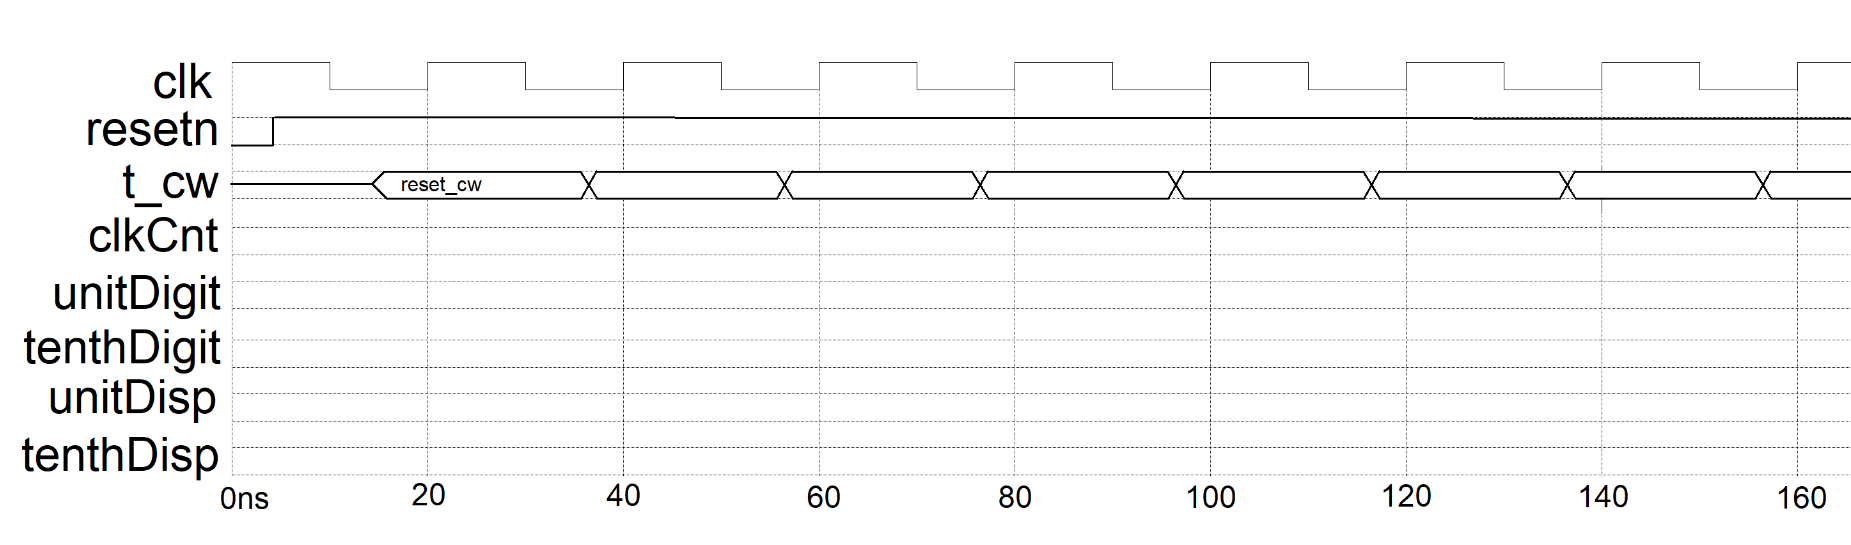
\includegraphics{ image4.png}

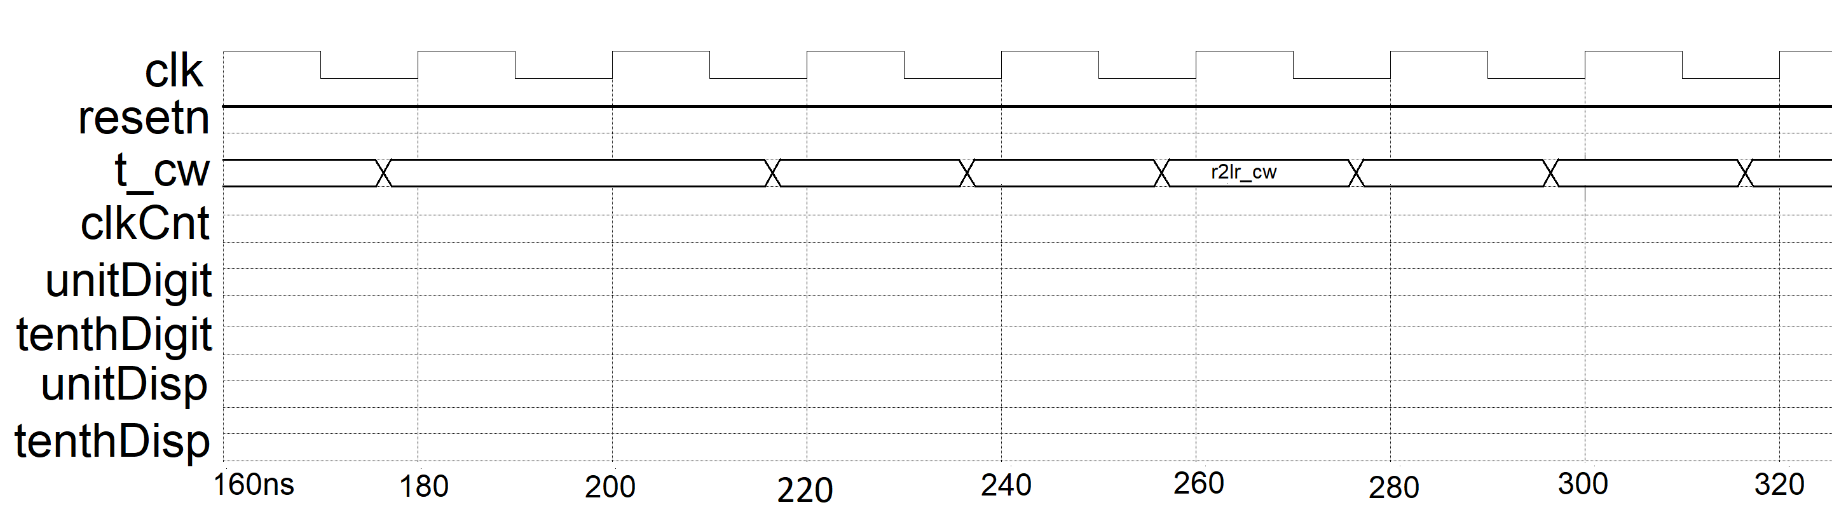
\includegraphics{ image5.png}

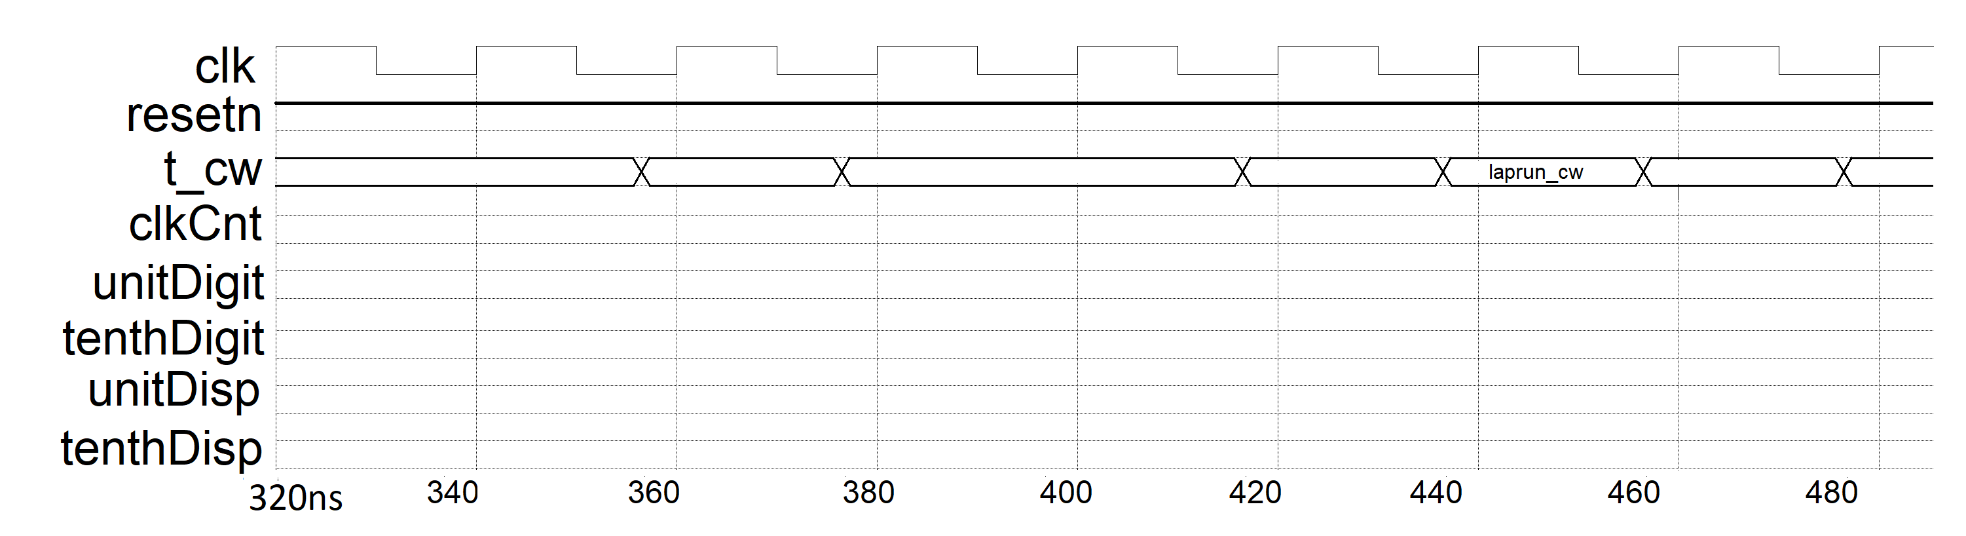
\includegraphics{ image6.png}

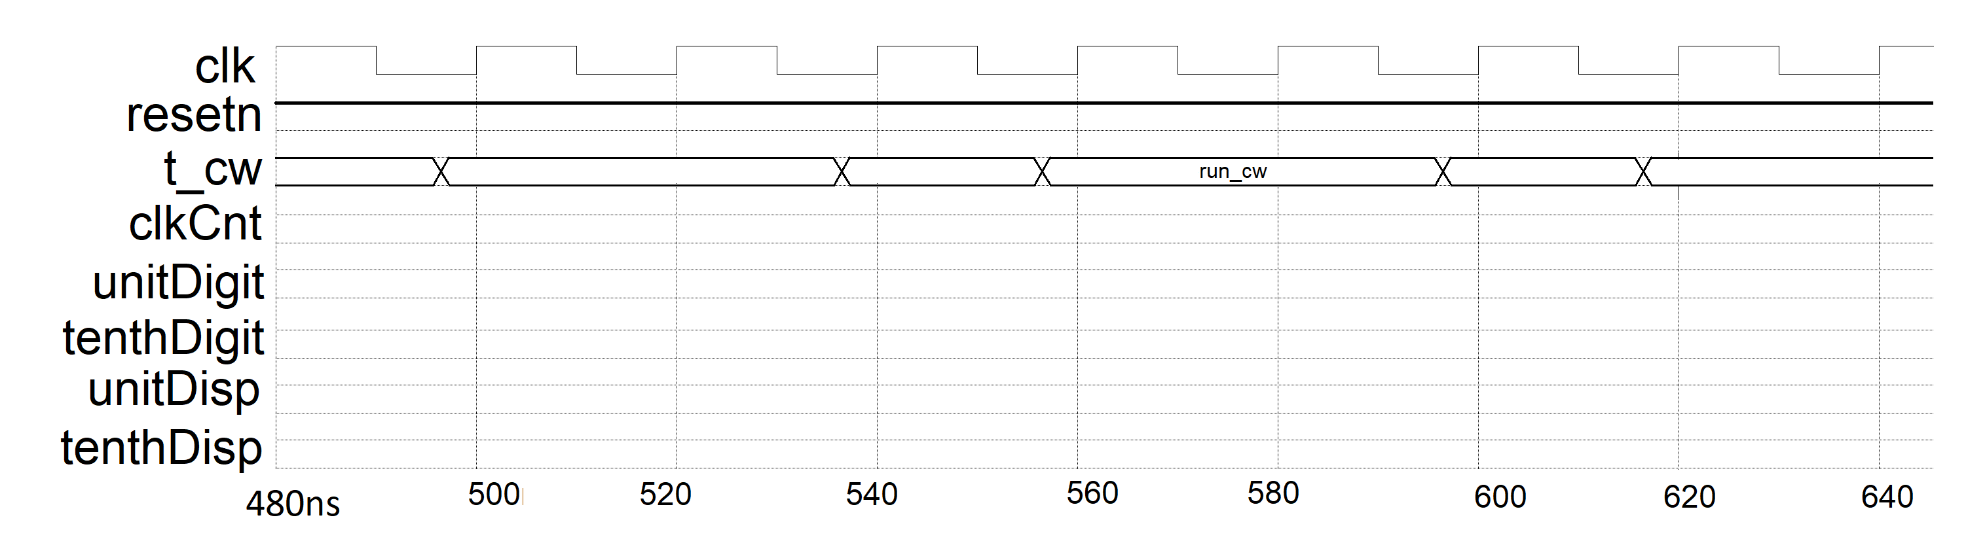
\includegraphics{ image7.png}

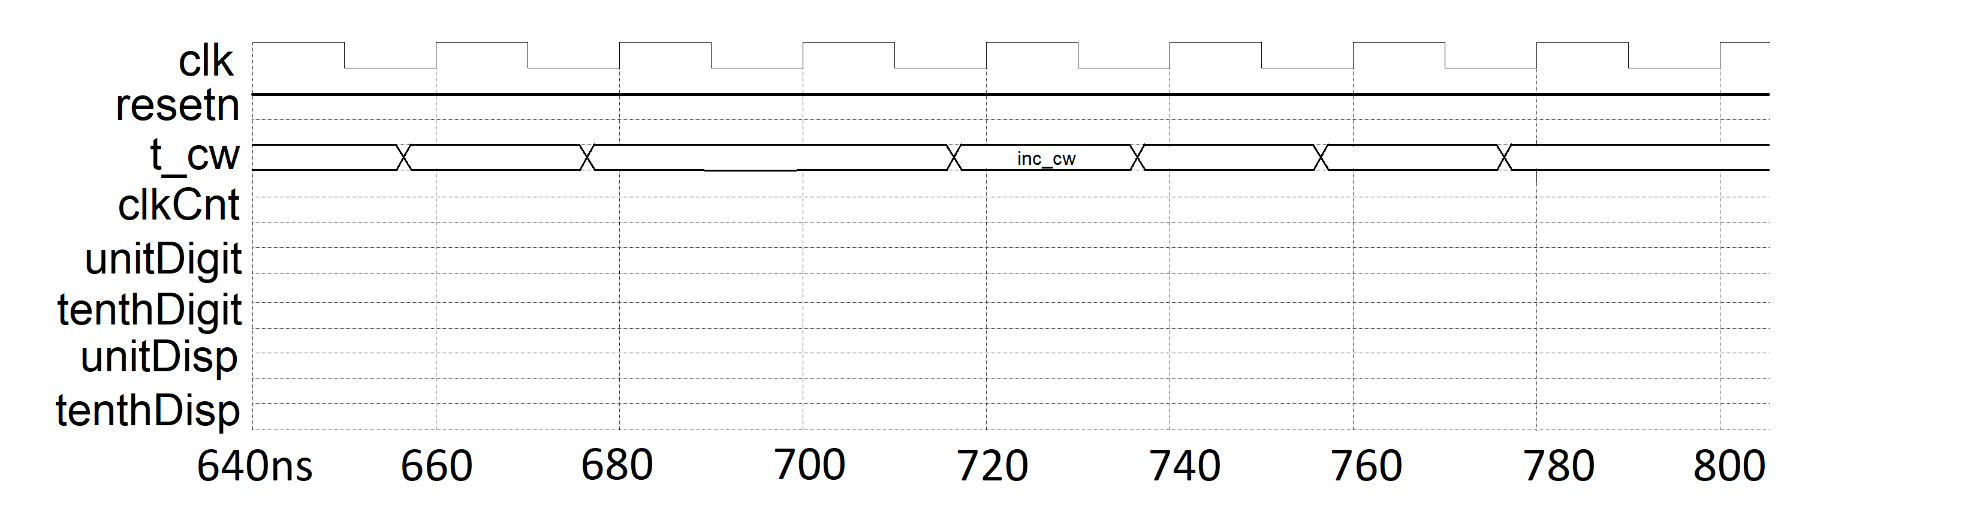
\includegraphics{ image8.png}

\begin{figure}[ht]
\caption{Complete the timing diagram using the control words found in the testbench.}
\label{figure:swDPtiming}
\end{figure}

\end{landscape}

\hypertarget{link:swDpSim}{}{{}
Before running the simulation, you need to complete the
do file given to you on Canvas.  Organize the waveforms
on your simulation as follows. 

\begin{tabular}{p{3cm}p{3cm}p{3cm}}
signal & radix & trace color \\ \hline
  clk 		& default 	& green  \\
  resetn 		& default 	& green  \\
  cw 		& hex 		& yellow  \\
  tenth 		& default 	& gold  \\
  clkCnt 		& hex 		& red  \\
  tenthDigit 	& hex 		& green  \\
  tenthDisp 	& hex 		& green  \\
  unitDigit 	& hex 		& greenyellow  \\
  unitDisp 	& hex 		& greenyellow  \\
\end{tabular}

Once you have the do file complete, launch the testbench
simulation in ModelSim and compare the expected output 
from Figure~\ref{figure:swDPtiming} against the actual 
output from your simulation.  Since you will not be synthesizing
your design, you need to ensure \underline{perfect} functionality
as you will use this module in an upcoming lab.  Do this by
looking for discrepancies starting at time 0 and only advancing 
the simulation when everything is correct. You will
have to transcend the design hierarchy to find the source of your
errors. Most errors are due to incorrect wiring of modules --
wrong signal names or wrong signal order. 

To get you started, your simulation output should look something like
the following.
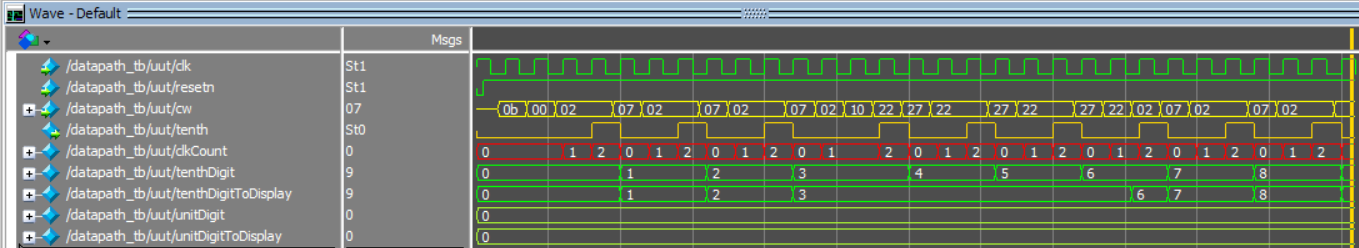
\includegraphics{ image10.png}

\section{Turn in}

You may work in teams of at most two. Make a record of your response to
the items below and turn them in a single copy as your team's solution
on Canvas using the instructions posted there. Include the names of both
team members at the top of your solutions. Use complete English
sentences to introduce what each of the following listed items (below)
is and how it was derived. In addition to this submission, you will be
expected to demonstrate your circuit at the beginning of your lab
section next week.

\subsubsection{System Architecture}

\begin{itemize}
\item
  Complete Table~\ref{table:swDPcontrolWord}.
\item
  \hyperlink{link:swDpVerilog}{Verilog code} for the body of the datapath module (courier 8-point font
  single spaced), leave out header comments.
  \end{itemize}
  
 \subsubsection{Testbench}
 \begin{itemize}
\item
 Complete timing diagram from Figure~\ref{figure:swDPtiming}.
\item
  A copy of your \hyperlink{link:swDpSim}{simulation timing} diagram. Use the signal
  color and order specified.
\item
  Demonstrate that your simulation to a member of the lab team.
\end{itemize}

